% =====================================================================
%  Khung ban thao — IEEE Networking Letters (gioi han 5 trang; <=4 trang MIEN PHI).
%
%  Chay `bash figures/build.sh` TRUOC, vi ban thao \input cac tep sinh ra:
%    figures/out/numbers.tex   macro so (mo hinh + do duoc + suy ra)
%    figures/out/captions.tex  loi hinh
%    figures/out/tab*.tex      bang
%
%  Dich: pdflatex main && bibtex main && pdflatex main && pdflatex main
% =====================================================================
\documentclass[journal]{IEEEtran}

\usepackage{graphicx}
\usepackage{amsmath}
\usepackage{booktabs}
\usepackage{url}

\graphicspath{{../figures/out/}}
%% SINH TU figures/make_figures.py -- KHONG sua tay.
\newcommand{\numFramePayload}{102}
\newcommand{\numCoapBlock}{64}
\newcommand{\numDtlsRT}{2}
\newcommand{\numMsgOneClassic}{37}
\newcommand{\numMsgOnePQ}{1192}
\newcommand{\numMsgTwoPQ}{4415}
\newcommand{\numExchOnePQ}{19}
\newcommand{\numExchTwoPQ}{69}
\newcommand{\numExchTotalPQ}{140}
\newcommand{\numKemFiveOneTwo}{800}
\newcommand{\numMOneMatch}{7}
\newcommand{\numMOneTotal}{7}
\newcommand{\numMOneImpl}{aiocoap 0.4.17}
\newcommand{\numGnutlsOk}{17}
\newcommand{\numGnutlsTotal}{21}
\newcommand{\numGnutlsAtFrame}{1/3}
\newcommand{\numGnutlsFragOk}{23}
\newcommand{\numGnutlsFragBad}{28}
\newcommand{\numMbedtlsOk}{14}
\newcommand{\numMbedtlsTotal}{14}
\newcommand{\numMbedtlsAtFrame}{2/2}
\newcommand{\numOpensslOk}{9}
\newcommand{\numOpensslTotal}{21}
\newcommand{\numOpensslAtFrame}{0/3}
\newcommand{\numOpensslMtuBad}{250}
\newcommand{\numOpensslMtuOk}{300}
\newcommand{\numKemFrameRatio}{7.8}
\newcommand{\numDecompError}{4.2}
\newcommand{\numBestBlock}{1024}
\newcommand{\numBestExch}{11}
\newcommand{\numBestRatio}{5.5}
\newcommand{\numQBlockMaxPayloads}{10}
\newcommand{\numQBlockExch}{15}
\newcommand{\numQBlockGain}{9.3}
\newcommand{\numFramePayloadSecured}{81}
\newcommand{\numMacOverhead}{25}
\newcommand{\numFramePayloadFrame}{127}
\newcommand{\numLinkSec}{21}
\newcommand{\numFragHdr}{5}
\newcommand{\numExchLo}{135}
\newcommand{\numExchHi}{147}
\newcommand{\numDirDefault}{280}
\newcommand{\numDirBest}{22}
\newcommand{\numDirQBlock}{30}
\newcommand{\numRatioDefault}{47}
\newcommand{\numRatioBest}{4}
\newcommand{\numRatioQBlock}{5}
\newcommand{\numFramesDefault}{280}
\newcommand{\numRatioFramesDefault}{2.43}
\newcommand{\numRatioFrames}{1.15}
\newcommand{\numBestFrames}{132}
\newcommand{\numGnutlsCapKB}{2.3}
\newcommand{\numMbedtlsMaxFrag}{32}
\newcommand{\numOpensslFewFragFail}{5}
\newcommand{\numOpensslManyFragOk}{19}
\newcommand{\numDtlsMeasTurns}{6}
\newcommand{\numDtlsMaxFrag}{94}
\newcommand{\numDtlsMinFrag}{32}
\newcommand{\numDtlsDatagramLo}{55}
\newcommand{\numDtlsDatagramHi}{115}
\newcommand{\numDtlsDatagramGrowth}{2.09}
\newcommand{\numDtlsImpl}{mbedtls 3.6.2}
\newcommand{\numDtlsMeasVersion}{1.2}
\newcommand{\numChainKeyBits}{8192}
\newcommand{\numSpanOk}{22.4}
\newcommand{\numSpanBad}{22.95}
\newcommand{\numSpanCells}{30}
\newcommand{\numSpanCerts}{3}
\newcommand{\numSpanMtus}{10}
\newcommand{\numSpanTrials}{150}
\newcommand{\numSpanCapKB}{2.3}
\newcommand{\numAmbiguousFrag}{23}
\newcommand{\numLongAllowance}{240}
\newcommand{\numLongRuns}{18}
\newcommand{\numLongSelfExit}{18}
\newcommand{\numLongKilled}{0}
\newcommand{\numLongSeconds}{46}
\newcommand{\numRelayCtrlCells}{30}

%% SINH TU figures/make_figures.py -- KHONG sua tay.
\newcommand{\capSizeRatio}{Lợi thế kích thước của EDHOC so với DTLS 1.3 trên chín bộ tham số NIST. Đường đứt: tỉ số cổ điển ở chế độ chữ ký (4.14$\times$). Đường chấm: chế độ Static DH (8.85$\times$), chế độ này KHÔNG có bản hậu lượng tử vì method 1--3 của RFC 9528 dựa trên Diffie--Hellman tĩnh.}
\newcommand{\capExchanges}{Số lượt trao đổi theo kích thước bản tin bắt tay. EDHOC trên CoAP dùng block-wise lock-step nên số lượt nở tuyến tính; DTLS 1.3 truyền theo flight nên giữ nguyên 2 lượt bất kể kích thước [RFC 9147]. Vòng tròn rỗng là SỐ ĐO trên một cài đặt CoAP độc lập, khớp mô hình 7/7. Con số của DTLS là trích chuẩn, không đo ở đây.}
\newcommand{\capBlocksize}{Quét toàn dải cỡ khối mà RFC 7959 cho phép, với bắt tay ML-KEM-768 + ML-DSA-65. Sao là điểm tối ưu của từng đường. Vùng tô và vạch dọc ở 64 B là TRẦN BIÊN DỊCH của RIOT (\texttt{CONFIG\_NANOCOAP\_BLOCK\_SIZE\_MAX}); cỡ khối bên phải vạch không dùng được nếu không sửa firmware. Hai bảng có điểm tối ưu KHÁC NHAU, nên không tồn tại một cấu hình tốt nhất chung cho cả độ trễ lẫn năng lượng.}
\newcommand{\capImplementations}{Ba cài đặt DTLS trên đường truyền ràng buộc; vạch chấm là payload một khung IEEE 802.15.4 (102 B). Số ô bắt tay thành công: gnutls 17/21; mbedtls 14/14; openssl 9/21. Ba cài đặt bị chặn bởi ba thứ khác nhau, nên kết quả này nói về TỪNG CÀI ĐẶT chứ không về giao thức DTLS.}
\newcommand{\capPerMessage}{Kích thước từng bản tin EDHOC. Đường đứt là payload một khung 802.15.4 (102 B). Cột giữa là SÀN của lập luận: biến thể hậu lượng tử nhẹ nhất có thể hình dung, chỉ ML-KEM-512 với xác thực cổ điển và chứng thư theo tham chiếu. Ngay ở sàn đó, riêng khoá đóng gói đã là 800 B, tức 7.8 lần payload khung, nên block-wise bị kích hoạt ngay ở message\_1 với mọi thiết kế.}


\begin{document}

\title{Does the Lightweight Handshake Stay Lightweight?\\
EDHOC, DTLS~1.3 and Post-Quantum Credentials on IEEE~802.15.4 Links}
\author{(authors withheld for now)}

\maketitle

\begin{abstract}
% ⛔ CHUA VIET. Cho toan van Fedrecheski de lay luan cu mo dau.
Placeholder.
\end{abstract}

\begin{IEEEkeywords}
EDHOC, DTLS, post-quantum cryptography, CoAP, IEEE 802.15.4, constrained devices.
\end{IEEEkeywords}

% =====================================================================
\section{Introduction}
% ⛔ CHUA VIET. Chan boi: can toan van Fedrecheski (WCNC 2024) de trich
% con so x6-x14 kich thuoc goi doi lai chi x1.44 thoi luong bat tay.
Placeholder.

% =====================================================================
% =====================================================================
%  PHAN KET QUA — dong gop CHINH cua bai.
%
%  ⚠ KHONG GO SO NAO VAO DAY. Moi con so den tu figures/out/numbers.tex,
%  do figures/make_figures.py sinh ra tu analysis/model.py va results/*.json.
%  Neu can mot so chua co macro thi THEM MACRO, dung go tay.
%
%  Chay `bash figures/build.sh` truoc khi dich ban thao.
% =====================================================================

\section{Measurement Setup}
\label{sec:setup}

All measurements run on a single machine (Ubuntu~24.04) so that every number in this letter
comes from one environment. Two quantities are measured, and neither requires a post-quantum
library: the argument is about message \emph{size}, so credentials are padded or substituted to
post-quantum dimensions rather than computed.

\textbf{Exchanges.} A relay placed between a CoAP client and server counts UDP datagrams in
each direction. Counting datagrams on the wire, rather than invocations inside the server,
matters: the implementation used here caches an assembled body and slices it, so a handler is
called once regardless of how many blocks cross the link.

\textbf{Handshake completion.} A DTLS client and server are run at a fixed MTU with
certificates of increasing size, and a handshake is recorded as complete only on evidence that
a successful run alone can produce, never on the absence of an error. Every implementation is
first exercised against each credential at a wide MTU; a pair that cannot complete there is
excluded rather than swept, since its cells would report a limit of the library rather than of
the link. This excluded one pair, discussed in Section~\ref{sec:threats}.

The block size is fixed at \numCoapBlock~B, the default in both Contiki-NG and RIOT, and the
constrained MTU is \numFramePayload~B, the payload of an IEEE~802.15.4 frame after the MAC
header and AES-CCM$^*$.

\section{Results}
\label{sec:results}

\subsection{The exchange count model agrees with an independent implementation}

Table~\ref{tab:validation} compares the exchange counts predicted by the block-wise model
against datagrams measured with \numMOneImpl, an implementation independent of the model:
\numMOneMatch/\numMOneTotal{} cases agree exactly. This validates the \emph{counting}, and
nothing more. It says nothing about latency or energy on a real link, neither of which is
claimed here.

With that model, a post-quantum EDHOC handshake at ML-KEM-768 and ML-DSA-65 takes
\numExchTotalPQ{} exchanges: \numExchOnePQ{} for message\_1 alone, whose \numMsgOnePQ~B do not
fit in a \numFramePayload~B frame. Fig.~\ref{fig:exchanges} shows the growth.

\subsection{The DTLS comparator, measured rather than cited}

DTLS fragments at its own handshake layer and sends each flight back-to-back, so its
round-trip count should not grow with size \cite{rfc9147}. We measure this rather than assume
it, at the same MTU and with the same relay. Certificate \emph{chains} are used to enlarge the
handshake without enlarging the key, since the library rejects keys beyond its configured
maximum integer size (Section~\ref{sec:threats}).

Across \numDtlsMinFrag{} to \numDtlsMaxFrag{} fragments, \numDtlsImpl{} completes every
handshake, and the datagram count grows from \numDtlsDatagramLo{} to \numDtlsDatagramHi{}
($\times\numDtlsDatagramGrowth$) while the number of direction changes stays at
\numDtlsMeasTurns{} throughout. The flight structure is therefore not an idealisation: at
\numDtlsMaxFrag{} fragments, more than twice what a post-quantum handshake requires, the
round-trip count has not moved.

Two qualifications matter. The measurement is DTLS~\numDtlsMeasVersion, because none of the
three implementations offers DTLS~1.3 over datagrams: GnuTLS lists protocol versions up to
DTLS~1.2 only, mbedTLS accepts \texttt{tls12}, \texttt{dtls12} and \texttt{tls13} but no
\texttt{dtls13}, and OpenSSL's \texttt{s\_server} has no DTLS~1.3 option. Four years after
RFC~9147, the two-round-trip figure it specifies is not obtainable from any of them. And the
constant here is \numDtlsMeasTurns{} direction changes rather than the \numDtlsRT{} round
trips of DTLS~1.3, since DTLS~1.2 carries more flights; what is measured is the invariance,
not the constant's value.

The threshold, not the ratio, is what matters. Classically an EDHOC message fits inside one
frame and block-wise never engages, so both protocols take \numDtlsRT{} round trips and
EDHOC's advantage is expressed purely in bytes. The ML-KEM-512 encapsulation key alone is
\numKemFiveOneTwo~B, which is $\numKemFrameRatio\times$ that frame payload, so block-wise engages in
message\_1 at every NIST parameter set, whatever authentication is chosen. This is a property
of transmitting a KEM public key, not of a particular design.

\subsection{Three implementations, three different limits}

Table~\ref{tab:impls} and Fig.~\ref{fig:impls} report whether each implementation completes a
DTLS handshake as MTU and certificate size vary. The three do not merely differ in degree;
they are bounded by different quantities.

\textbf{OpenSSL is bounded by MTU.} It fails at every MTU at or below \numOpensslMtuBad~B and
completes at every MTU at or above \numOpensslMtuOk~B, for all three certificate sizes. The
boundary sits at OpenSSL's \texttt{DTLS1\_MIN\_MTU} of 256~B. Fragment count explains nothing
here: it fails with \numOpensslFewFragFail{} fragments at MTU~\numOpensslMtuBad{} and completes with \numOpensslManyFragOk{} at MTU~\numOpensslMtuOk{}. At the
\numFramePayload~B payload of an 802.15.4 frame it completes \numOpensslAtFrame{} cases, which
is to say none. \textbf{This holds for classical credentials too}; it is not a post-quantum
result.

\textbf{GnuTLS is bounded by fragment count.} It completes at MTU~\numFramePayload, so no MTU
floor applies, but it completes up to \numGnutlsFragOk{} fragments and fails from
\numGnutlsFragBad{}. The failures are not an artefact of an impatient
harness: given an allowance far beyond the probe timeout, the client still
abandons the handshake on its own retransmission schedule, well inside that allowance. At
\numFramePayload~B, \numGnutlsFragOk{} fragments cap a handshake message at about
\numGnutlsCapKB~kB, which post-quantum credentials exceed.

\textbf{mbedTLS shows neither limit} in the range swept, completing
\numMbedtlsOk/\numMbedtlsTotal{} cases including \numMbedtlsAtFrame{} at
MTU~\numFramePayload{} with \numMbedtlsMaxFrag{} fragments.

This ordering is worth stating plainly. Of the three, mbedTLS is the one actually deployed on
constrained devices, and it is the one that handles the constrained link; the two
server-side implementations do not. The expectation that motivated this measurement was the
opposite.

\subsection{No block size recovers the round trips}

The obvious objection to Section~\ref{sec:results} is that the block size is a tunable
parameter. Fig.~\ref{fig:blocksize} sweeps the full range RFC~7959 permits. Larger blocks do
reduce the exchange count, but each block then exceeds the frame and is fragmented by the
adaptation layer, where a lost fragment costs the whole block~\cite{rfc4944,rfc6282}. RFC~9177~\cite{rfc9177} defines
alternative block options, and dismissing them because no constrained stack implements them
would state a structural conclusion on a contingent fact. We therefore model them.

Q-Block with non-confirmable messages sends blocks serially ``without having to wait for a
response or next request'', acknowledging them in sets of \numQBlockMaxPayloads{}, the default
value of \texttt{MAX\_PAYLOADS}~\cite{rfc9177}. The exchange count becomes the number of such
sets rather than the number of blocks: \numQBlockExch{} instead of \numExchTotalPQ{}, a
reduction of $\numQBlockGain\times$. So the option does recover most of what lock-step costs.

It does not close the gap. \numQBlockExch{} exchanges remain against the
\numDtlsMeasTurns{} direction changes measured for DTLS, and the recovery is unavailable in
practice: neither Contiki-NG nor RIOT implements Q-Block, libcoap gates it behind a flag that
both peers must set, and neither RFC~9528 nor RFC~9668 references RFC~9177. The conclusion this
letter draws is therefore about EDHOC as profiled in RFC~9668, not about every conceivable
CoAP transport for it. The optimum lies at the
boundary of the permitted range rather than inside it, at \numBestBlock~B, and even there the
count is \numBestExch{} exchanges against \numDtlsRT{} DTLS flights, a factor of
$\numBestRatio\times$.

Two further points close the objection. The optimum is not reachable on RIOT, whose
\texttt{CONFIG\_NANOCOAP\_BLOCK\_SIZE\_MAX} is a compile-time ceiling at \numCoapBlock~B; and
the latency-optimal and energy-optimal block sizes are not the same, so no single setting is
best on both axes.


% =====================================================================
% =====================================================================
%  DE DOA TOI TINH HOP LE.
%
%  Muc nay ton tai de KHAI TRUOC nhung gi phan bien se hoi. Luat cua nha:
%  ``chua mo hinh'' ma khong kem SO chi la mot loi xin loi. Nen moi han che o
%  day phai kem HOAC mot con so HOAC mot phat bieu kiem duoc.
%
%  ⚠ KHONG GO SO. Xem paper/check-no-typed-numbers.py
% =====================================================================

\section{Threats to Validity}
\label{sec:threats}

\textbf{No constrained hardware.} Every measurement here runs on a desktop over loopback. This
bounds what may be claimed, and the claims are bounded accordingly: exchange counts are a
property of the transport, and no statement is made about latency, energy, or memory. Those
have been measured on real hardware by others, for TLS and DTLS over
6TiSCH~\cite{claeys2021}, for an embedded EDHOC module~\cite{fraile2021}, and for
post-quantum EDHOC~\cite{fraile2025}; this letter cites rather than repeats them.
The one quantity that would change on real hardware, retransmission behaviour under loss, is
addressed only qualitatively.

\textbf{One implementation excluded, not reported as a failure.} mbedTLS cannot load the
largest certificate at all: \texttt{mbedtls\_x509\_crt\_parse\_file} rejects the key, which
exceeds the library's configured maximum integer size. Its cells for that credential would
otherwise read as failures at every MTU, including the widest, and would look exactly like a
result about the link. They are a limit of the library, reached before the link is touched.
The per-pair control described in Section~\ref{sec:setup} exists for this case, and this is
the pair it removed.

\textbf{Findings are about implementations, not about DTLS.} The three libraries are bounded
by different quantities at very different points, so nothing here supports a statement about
the protocol. Where DTLS~1.3 itself is characterised, in particular its constant round-trip
count, the source is the specification \cite{rfc9147} and not these measurements. No DTLS~1.3
implementation was available to us; \texttt{s\_server} in the OpenSSL version used still
offers no DTLS~1.3 option, so the flight behaviour was exercised on DTLS~1.2, where the
mechanism is the same and only the flight count differs.

\textbf{Loss is assumed independent.} The block-size sweep treats frame losses as independent,
which is optimistic for a low-power radio: bursty loss favours larger blocks, and would move
the optimum. The conclusion drawn from that sweep is deliberately weaker than the curve
allows, namely that no permitted block size brings the exchange count near the DTLS flight
count, and this holds across the whole loss range plotted, including the lossless case.

\textbf{One estimated parameter.} The MAC and link-layer security overhead subtracted from the
frame is an estimate rather than a measurement. It affects the frame payload and so the
fragment counts. It cannot affect the threshold argument: the smallest standardised KEM
encapsulation key is $\numKemFrameRatio\times$ the frame payload, and no plausible correction
of a few bytes changes that.

\textbf{Scope is EDHOC over CoAP.} The lock-step behaviour follows from CoAP block-wise
transfer, so it applies to the profile of \cite{rfc9668} and not to EDHOC carried over some
other transport. The per-message decomposition reproduces the published total to within
\numDecompError\%, which is adequate for counting exchanges but not for quoting absolute
sizes; absolute sizes are taken from the published comparison instead.


% =====================================================================
\section{Conclusion}
% ⛔ CHUA VIET.
Placeholder.

% =====================================================================
% HINH VA BANG. Tat ca sinh ra, khong go tay.
\begin{figure}[t]
  \centering
  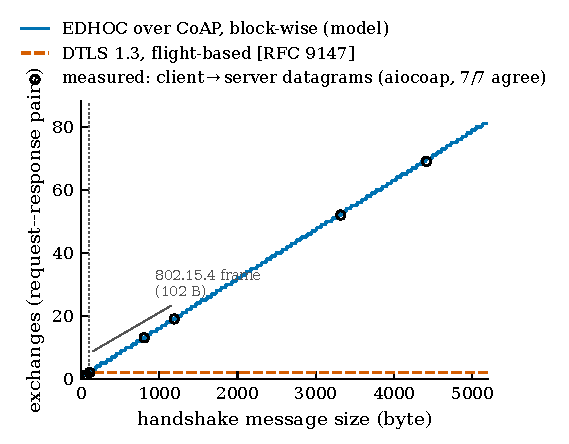
\includegraphics[width=\columnwidth]{fig2-exchanges.pdf}
  \caption{\capExchanges}
  \label{fig:exchanges}
\end{figure}

\begin{figure*}[t]
  \centering
  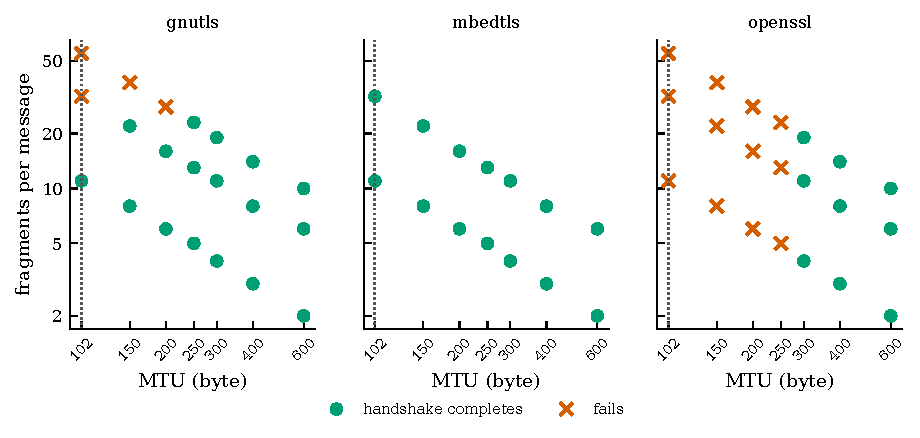
\includegraphics[width=\textwidth]{fig4-implementations.pdf}
  \caption{\capImplementations}
  \label{fig:impls}
\end{figure*}

\begin{figure*}[t]
  \centering
  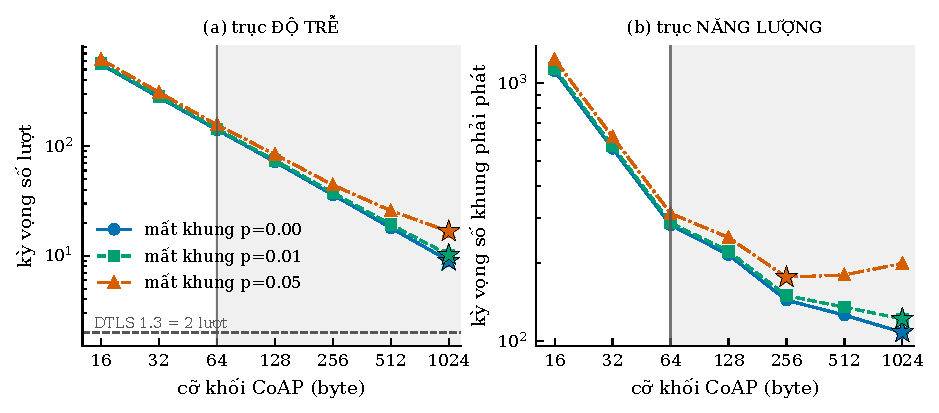
\includegraphics[width=\textwidth]{fig3-blocksize-tradeoff.pdf}
  \caption{\capBlocksize}
  \label{fig:blocksize}
\end{figure*}

%% SINH TU figures/make_figures.py -- KHONG sua tay.
\begin{table*}[t]
\centering
\caption{Exchange-count model against an independent CoAP implementation (aiocoap 0.4.17). Datagrams are counted by a UDP relay between client and server; 7/7 agree.}
\label{tab:validation}
\footnotesize
\begin{tabular}{lrrrc}
\hline
case & byte & model & measured & agree \\
\hline
EDHOC message 1, classical & 37 & 1 & 1 & yes \\
EDHOC message 2, classical & 111 & 2 & 2 & yes \\
EDHOC message 3, classical & 77 & 1 & 1 & yes \\
EDHOC message 1, ML-KEM-512 & 808 & 13 & 13 & yes \\
EDHOC message 1, ML-KEM-768 & 1192 & 19 & 19 & yes \\
EDHOC message 2, K768/D65 & 4415 & 69 & 69 & yes \\
EDHOC message 3, K768/D65 & 3322 & 52 & 52 & yes \\
\hline
\end{tabular}
\\[2pt]{\footnotesize Block size 64~B, engaging above 102~B. This validates the counting only; latency and energy are not measured here.}
\end{table*}

%% SINH TU figures/make_figures.py -- KHONG sua tay.
\begin{table*}[t]
\centering
\caption{Bounding quantity for each DTLS implementation. `Cells' counts configurations completing a handshake out of those swept; `at frame MTU' restricts that to MTU~102~B.}
\label{tab:impls}
\footnotesize
\begin{tabular}{llll}
\hline
implementation & cells & at frame MTU & bounded by \\
\hline
gnutls & 17/21 & 1/3 & spans \$\textbackslash\{\}le\$22.4 frame payloads (30 cells) \\
mbedtls & 14/14 & 2/2 & none found in range \\
openssl & 9/21 & 0/3 & MTU floor: 250 fails / 300 ok \\
\hline
\end{tabular}
\\[2pt]{\footnotesize The three are bounded by different quantities, so these results characterise the implementations and not the DTLS protocol.}
\end{table*}


\bibliographystyle{IEEEtran}
\bibliography{refs}

\end{document}
